\documentclass[dvisvgm]{standalone}

% Graphiken
\usepackage{tikz}

% TikZ Bibliotheken
\usetikzlibrary{
    arrows,
    arrows.meta,
    decorations,
    backgrounds,
    positioning,
    fit,
    petri,
    shadows,
    datavisualization.formats.functions,
    calc,
    shapes,
    shapes.multipart
}

\begin{document}
\textcolor{white}{workaround}
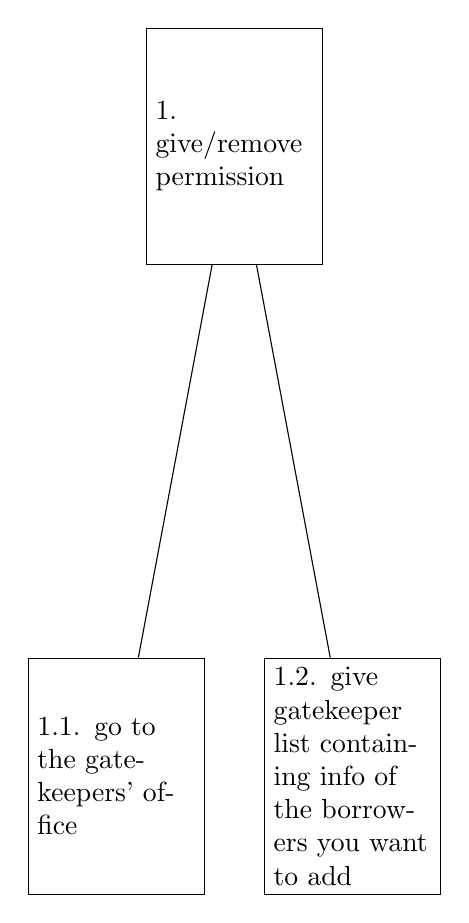
\begin{tikzpicture}[sibling distance=3cm, level distance=8cm]

  \node[
    draw,
    text width=2cm,
    minimum height=3cm
  ] at (0,-1)
  {1. give/remove permission}
    % 1.1. {{{
    child {
      node[
        draw,
        text width=2cm,
        minimum height=3cm
      ]
      {1.1. go to the gatekeepers' office}
    }
    % }}}
    % 1.2. {{{
    child {
      node[
        draw,
        text width=2cm,
        minimum height=3cm
      ]
      {1.2. give gatekeeper list containing info of the
        borrowers you want to add}
    };
    % }}}

\end{tikzpicture}
\end{document}
